\begin{frame}[label=tracers]
    \frametitle{Remote Sensing Require Tracers}
    \begin{tikzpicture}[remember picture, overlay]
        % background img
        \node[anchor=south east, inner sep=0pt] (img_bk) at ([yshift=0.5cm]current page.south east) {%
        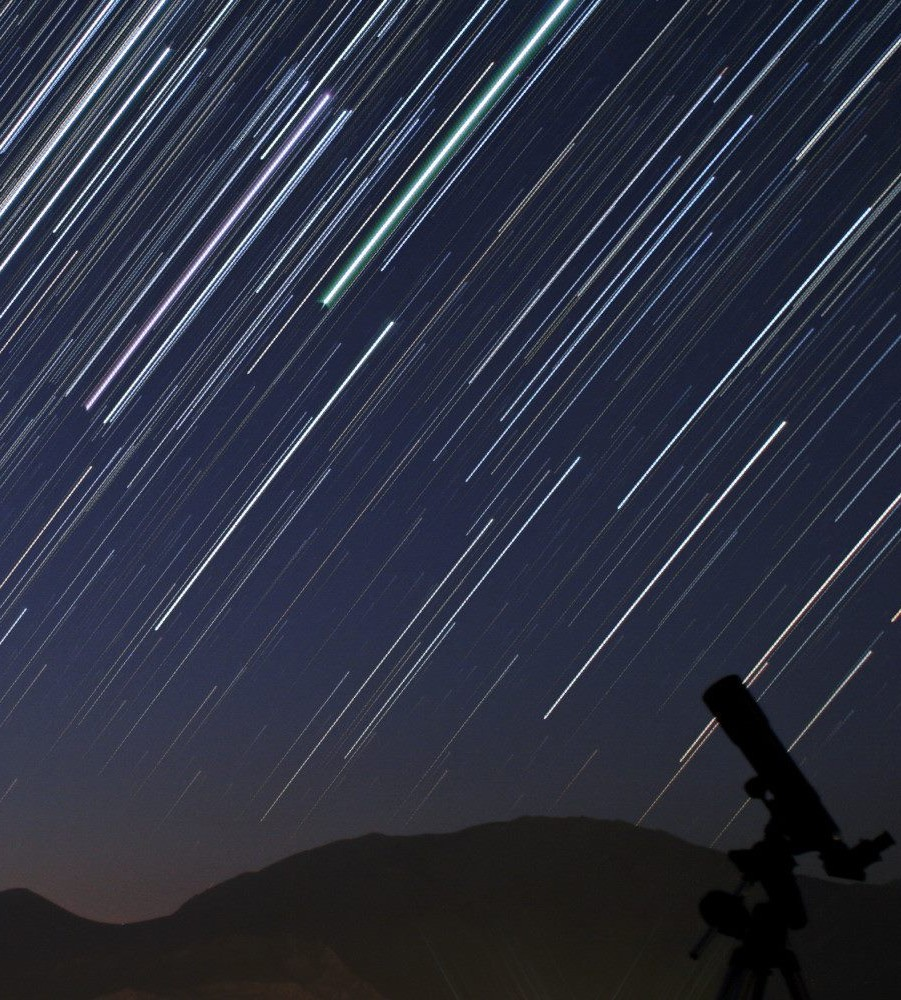
\includegraphics[height=\textheight - 1.1cm]{img/meteor_shower_cropped.jpg}
        };
        \node[anchor=south east, inner sep=0pt, text=white, xshift=-5pt, yshift=0.5cm] at (current page.south east) {%
        \tiny \textit{Credit:} \href{https://www.vox.com/2014/5/23/5744710/theres-a-big-meteor-shower-coming-tonight-heres-how-to-see-it}{\underline{Babek Tafreshi/SSPL/Getty Images}}
        };

        % glitter img
        \node<2->[anchor=north west, inner sep=2pt] (img) at (img_bk.north west) {
            {\includegraphics[height=0.2\textheight]{img/glitter/glitter1.png}}
        };
        \node<2->[anchor=south east, inner sep=2pt] at (img.south east) { 
            {{{\fontsize{3}{3.4}\selectfont\raggedleft \textcolor{white}{\textit{Credit}: \href{https://www.youtube.com/watch?v=5zI9sG3pjVU}{\underline{Veritasium (YT)}}}}}}
        };
        \node<2->[anchor=north, inner sep=2pt] at (img.south) { 
            {\centering \tiny \textcolor{white}{Glitter traces liquid turbulence}}
        };

        % laser img
        \node<3->[anchor=north east, inner sep=2pt] (img) at (img_bk.north east) {
            {\includegraphics[height=0.2\textheight]{img/laser/laser1.png}}
        };
        \node<3->[anchor=south east, inner sep=2pt] at (img.south east) { 
            {{{\fontsize{3}{3.4}\selectfont\raggedleft \textcolor{white}{\textit{Credit}: \href{https://www.youtube.com/watch?v=5zI9sG3pjVU}{\underline{Veritasium (YT)}}}}}}
        };
        \node<3->[anchor=north, inner sep=2pt] at (img.south) { 
            {\centering \tiny \textcolor{white}{Lasers trace air currents }}
        };

        % biker img
        \node<4->[anchor=north, inner sep=0pt] (img) at ([yshift=-0.3\textheight]img_bk.north) { 
            {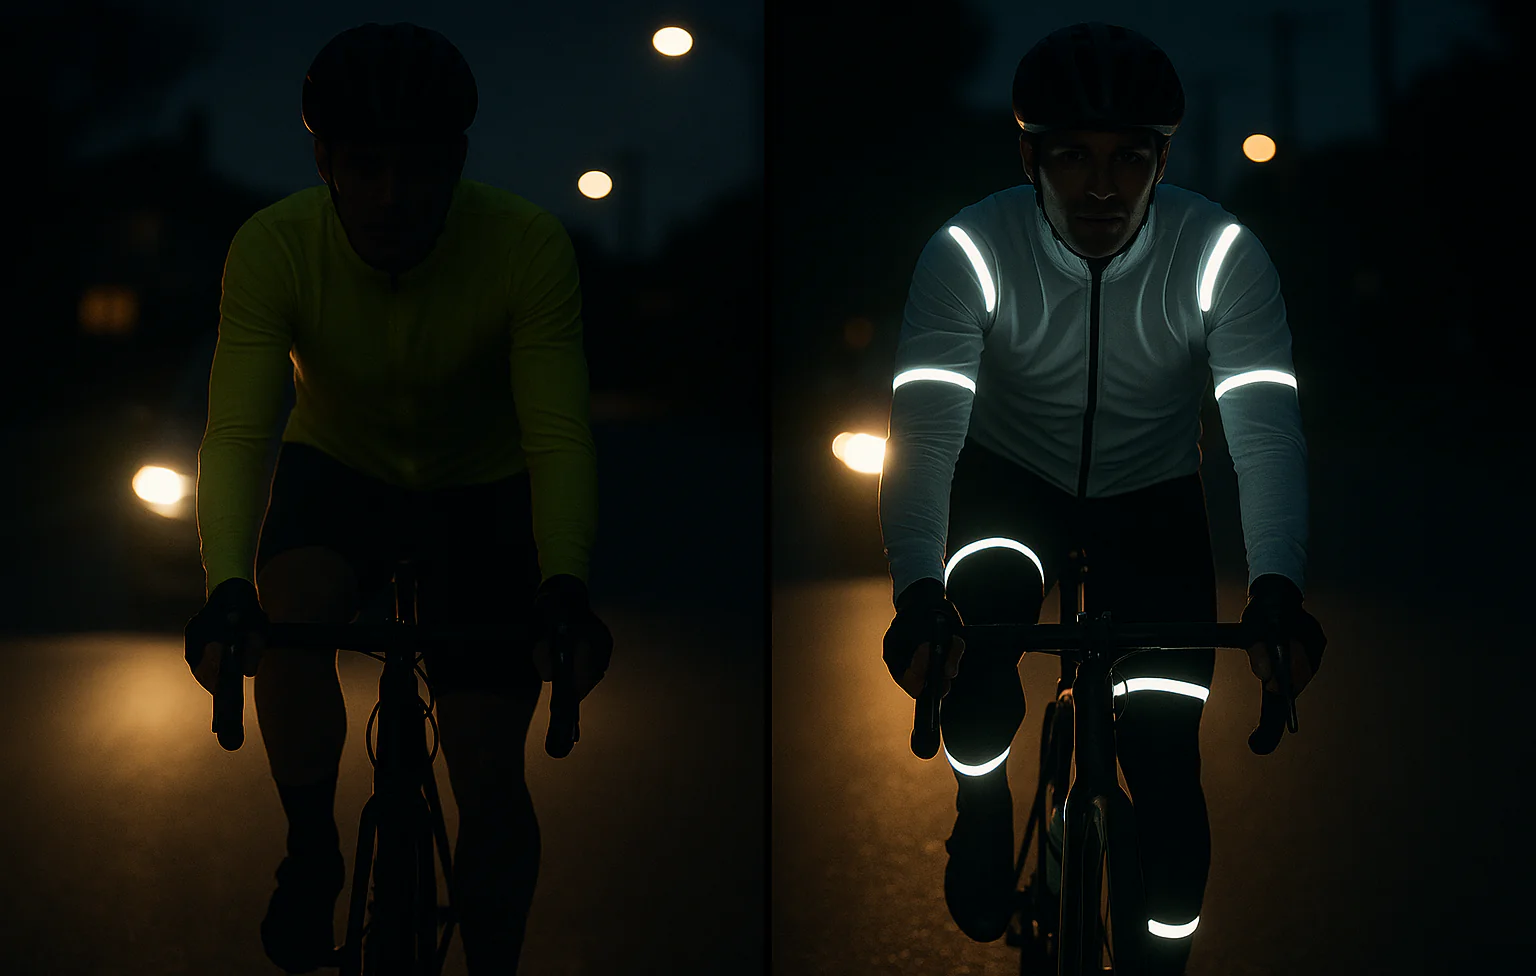
\includegraphics[height=0.2\textheight]{img/Retroreflective.png}}
        };
        \node<4->[anchor=south east, inner sep=2pt] at (img.south east) { 
            {{{\fontsize{3}{3.4}\selectfont\raggedleft \textcolor{white}{\textit{Credit:} \href{https://cdn.shopify.com/s/files/1/0056/6847/0855/files/Retroreflective.png?v=1747759064}{\underline{Shopify}}}}}}
        };
        \node<4->[anchor=north, inner sep=2pt] at (img.south) { 
            {\centering \tiny \textcolor{white}{Retroreflectors trace bicyclists }}
        };
    \end{tikzpicture}

    \begin{columns}
        \begin{column}{0.65\textwidth}
            \alert{Tracers} highlight quantities of interest

            \uncover<5->{\(\xrightarrow[]{}\) \colorbox{yellow}{Meteors make great high atmosphere tracers!}}
            ~\\ ~ \\

            \uncover<6->{Meteors happen all the time, everywhere! 
            \begin{itemize}
                \item Thousands per hour above your head
                \item Size: dust or sand
            \end{itemize}}

            \uncover<7->{Meteors leave a long \alert{plasma trail} as they burn up}
            \begin{itemize}
                \item<8-> Drifts in \textit{wind}
                \item<9-> Diffusion influenced by \textit{pressure, temperature}
                \item<10-> Trails are \alert{radar reflective}
            \end{itemize}
        \end{column}
        \begin{column}{0.4\textwidth}
            
        \end{column}
    \end{columns} 
    \centering
    ~\\ ~ \\ 
    \uncover<11->{\colorbox{yellow}{\textbf{No other way to densely sample this region's environment!}}}
\end{frame}